\documentclass[11pt,a4paper]{article}

\usepackage{titling}
\usepackage[hidelinks]{hyperref}
\usepackage{graphicx}
\usepackage{grffile}
\usepackage{float}
\usepackage{geometry}
\usepackage{listings}

\newcommand{\subtitle}[1]{
  \posttitle{
    \par\end{center}
    \begin{center}\large#1\end{center}
    \vskip0.5em}
}

\begin{document}
\title{Web Application User Manual}
\subtitle{ Git: \url{https://github.com/CodingInfinity/Benchmark-Service-Documentation} \\ GitHub Organisation: \url{https://github.com/CodingInfinity}}
\begin{figure}
			\centering
			
\includegraphics[height=230px]{../Images/CodingInfinity.png}
\end{figure}
\author{
	\textbf{The Client:} \\
	Ms Vreda Pieterse  \\
	Department of Computer Science \\
	University Of Pretoria
	\\
	\\
	\textbf{The Team:} \\
	Andrew Broekman		\emph{11089777}	\\
	Brenton Watt		\emph{14032644}	\\
	Fabio Loreggian		\emph{14040426}	\\
	Reinhardt Cromhout	\emph{14009936}	\\
}
\date{\textbf{May 2016}}

\maketitle
\thispagestyle{empty}
\pagebreak

\tableofcontents
\pagebreak
\section{Introduction}
This is the user manual for the Web Application. It gives a detailed guide surrounding individual how to
navigate and use each part of the system.

\section{Registration}
Upon starting up of the application and navigating to the home page, the user will be met with the screen seen in 
Figure \ref{fig:landPage}.
\begin{figure}[H]
	\begin{center}
		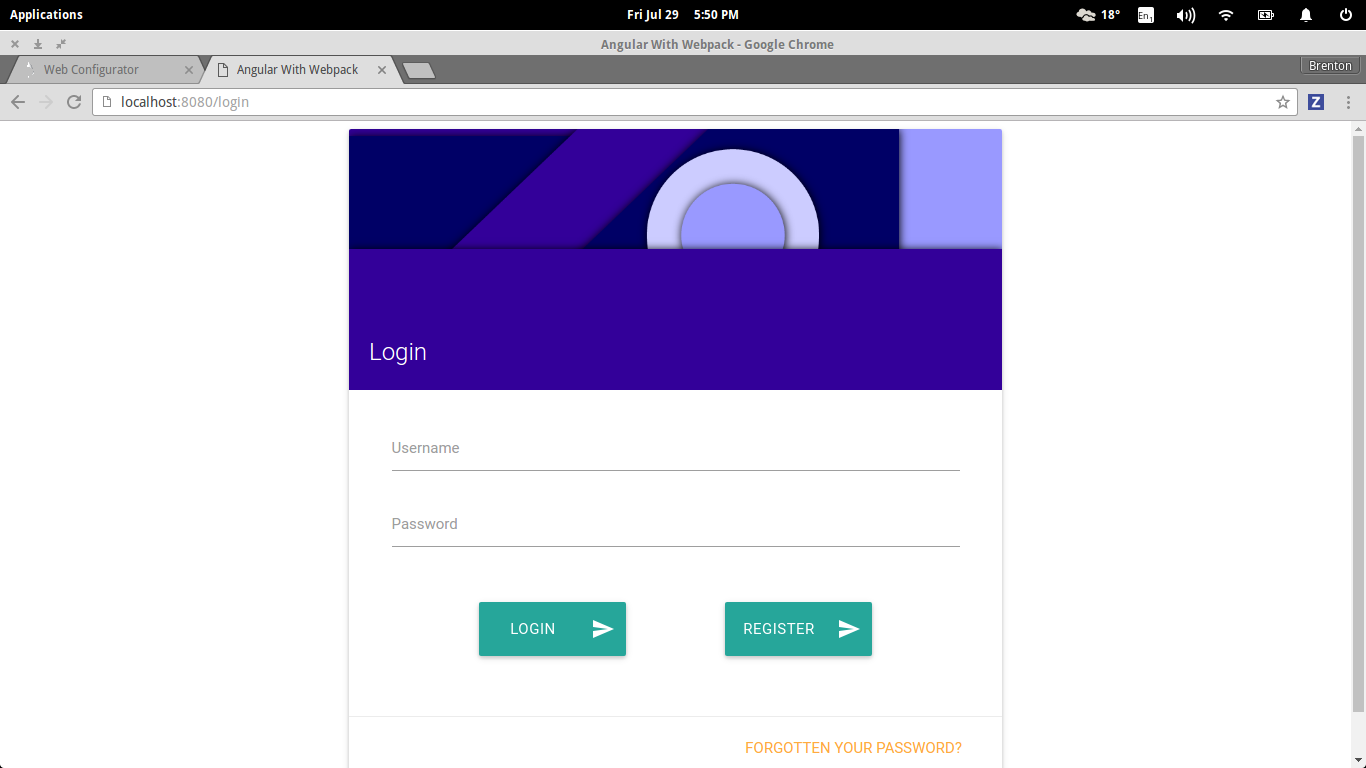
\includegraphics[scale=0.3]{../Images/User Manual/Landing Page.png}
		\caption{Landing Page}
		\label{fig:landPage}
	\end{center}  
\end{figure}

If the user has never made use of the system before, they should register themselves. Clicking on the "Register"
button will direct the user to the page seen in Figure \ref{fig:regPage}.
\begin{figure}[H]
	\begin{center}
		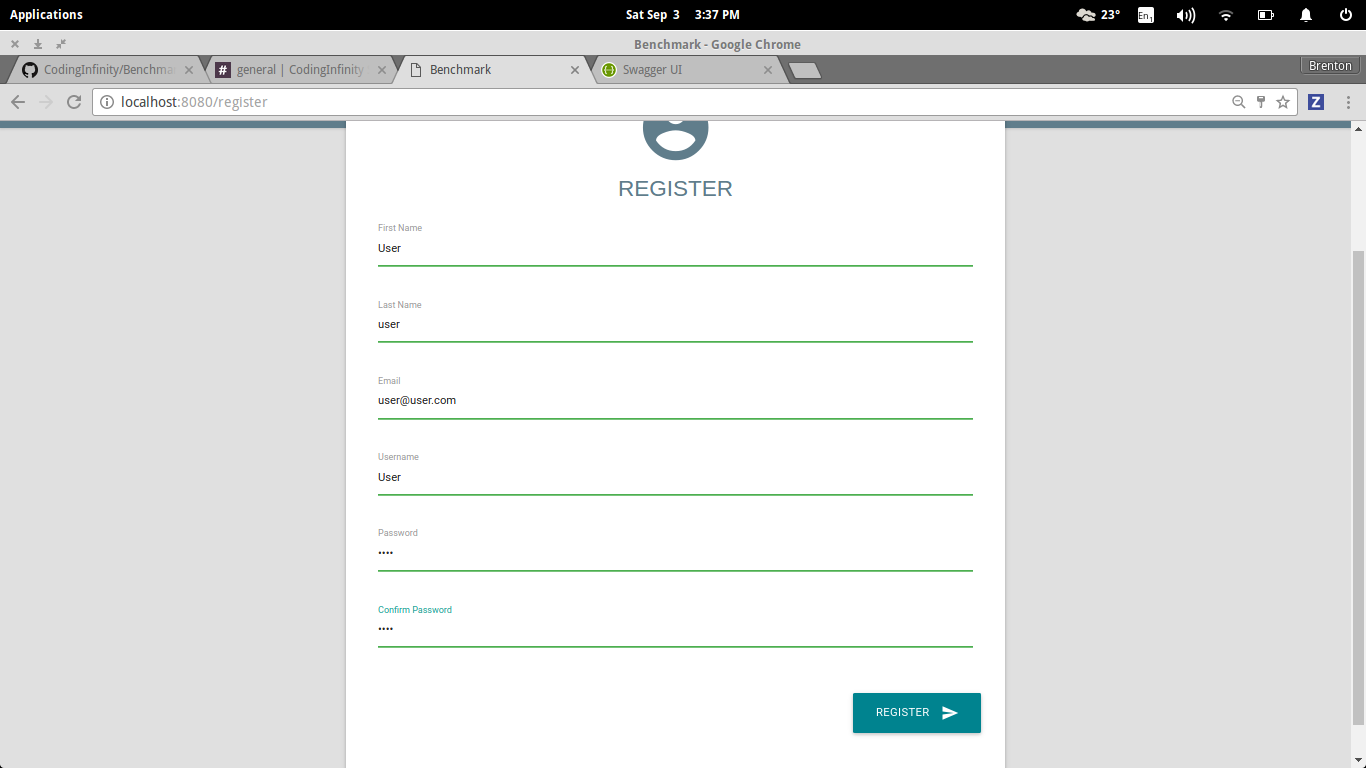
\includegraphics[scale=0.3]{../Images/User Manual/Registration Page.png}
		\caption{Registration Page}
		\label{fig:regPage}
	\end{center}  
\end{figure}

The user will then need to fill in their details accordingly. Once they have done this, they should click the "Submit" 
button. The user will then receive an email address at the address provided with a link that will allow them to activate
their account. When they click on the link they will arrive at a page as seen in Figure \ref{fig:activatePage}.
\begin{figure}[H]
	\begin{center}
		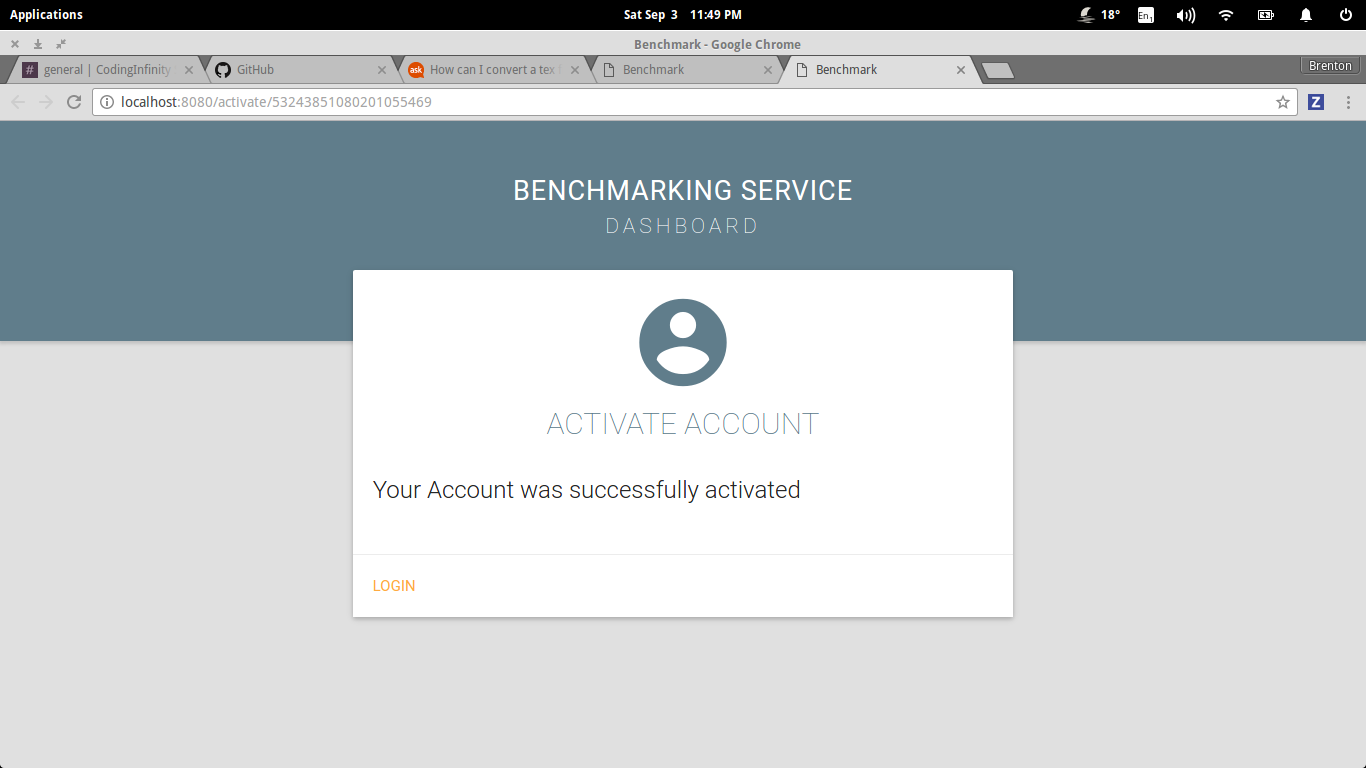
\includegraphics[scale=0.3]{../Images/User Manual/Activation Page.png}
		\caption{Activation Page}
		\label{fig:activatePage}
	\end{center}  
\end{figure}

\section{Sign In}
Once the user has registered and activated an account as detailed in the previous section or upon returning to the application,
they will be able to sign in by filling in their details as seen in Figure \ref{fig:signPage}.
\begin{figure}[H]
	\begin{center}
		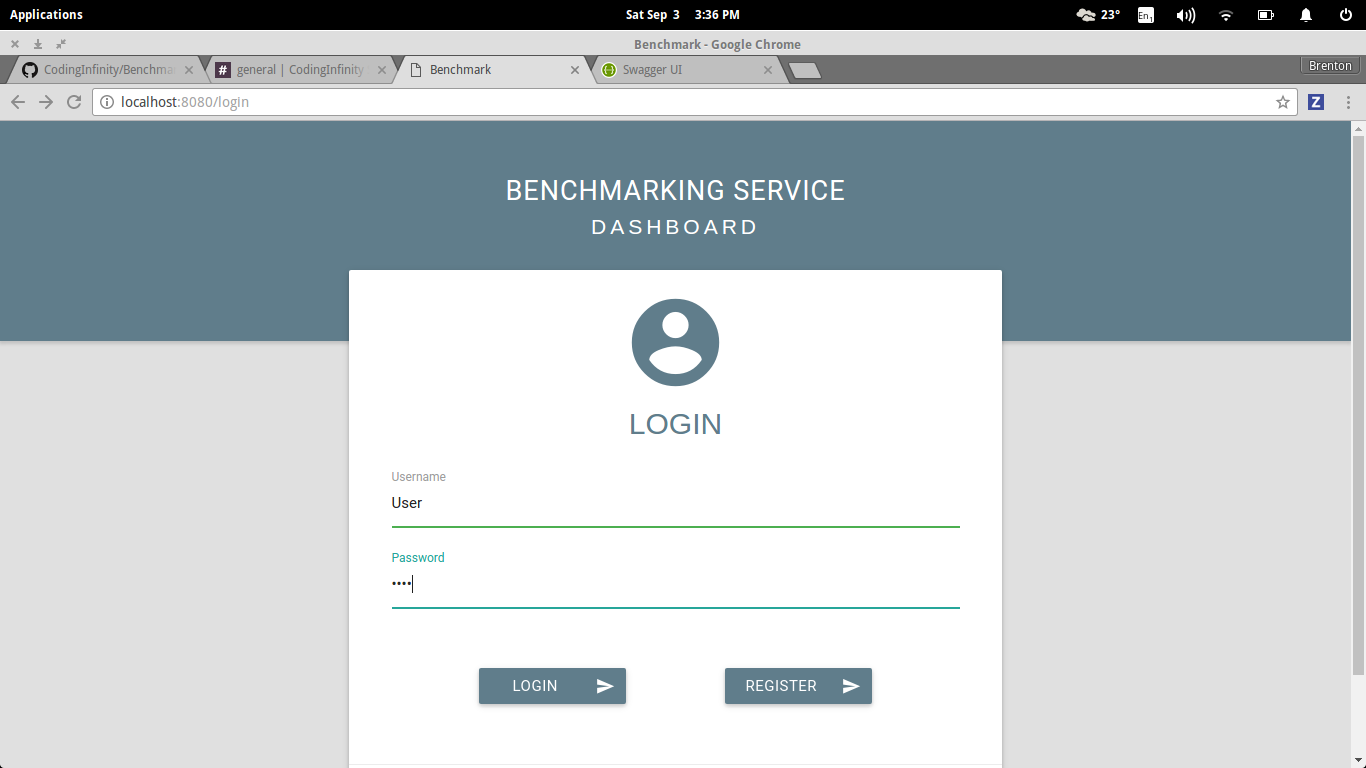
\includegraphics[scale=0.3]{../Images/User Manual/Sign in Page.png}
		\caption{Signing in}
		\label{fig:signPage}
	\end{center}  
\end{figure}

\section{Home}
Upon signing in, the user will arrive at the home page as seen in Figure \ref{fig:homePage}. From this page the user will be able 
to navigate throughout the application.
\begin{figure}[H]
	\begin{center}
		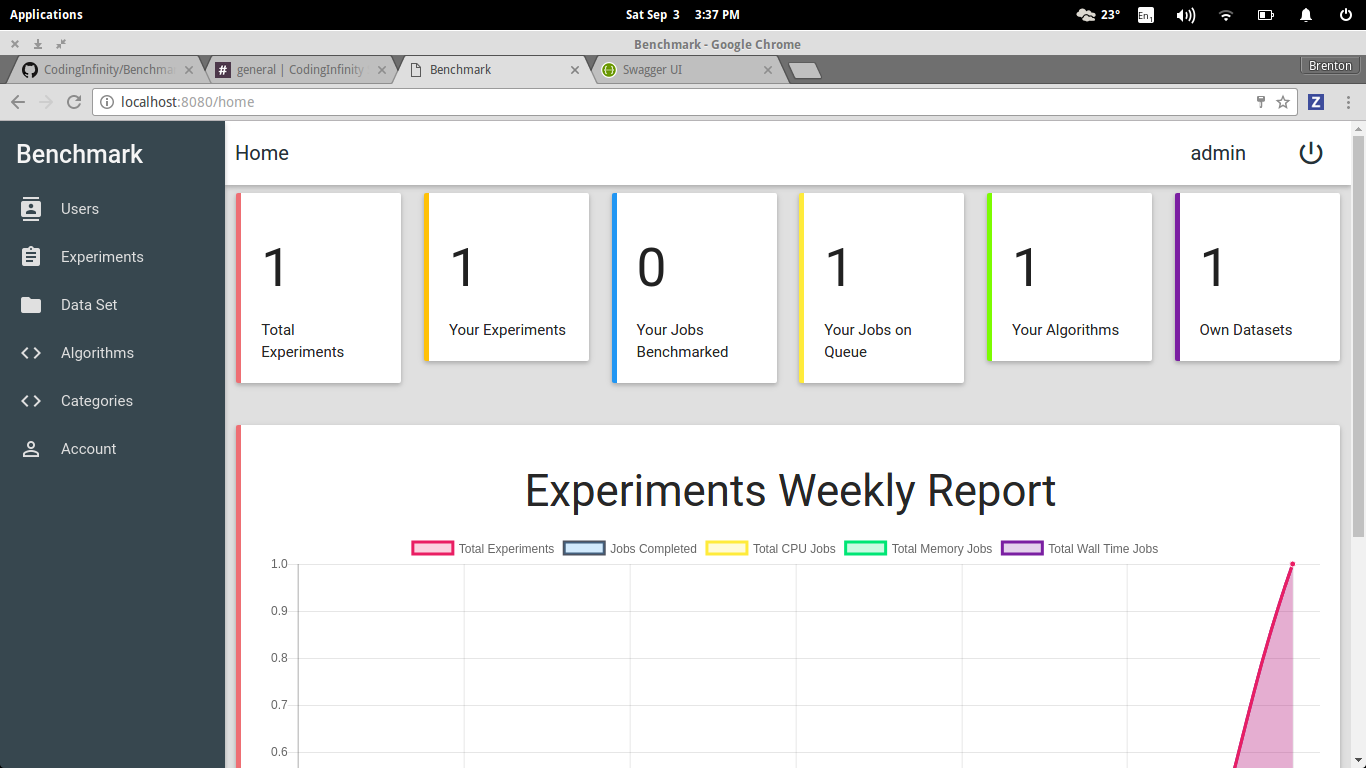
\includegraphics[scale=0.3]{../Images/User Manual/Home Page.png}
		\caption{Home Page}
		\label{fig:homePage}
	\end{center}  
\end{figure}
\section{Edit Profile}
In order to edit ones profile, click on the Account tab in the navigation bar and a drop down list will appear as seen in Figure \ref{fig:AccountPage}.
From there, click on the "Profile" option, which will take you to the Profile page as seen in Figure \ref{fig:ProfilePage}.
From here, the user can edit any of the options availible by clicking on the desired option and filling in the details as seen in
Figures \ref{fig:ProfilePage1}, \ref{fig:ProfilePage2}, \ref{fig:ProfilePage3}. Upon filling in the details, click the "Edit" button.
\begin{figure}[H]
	\begin{center}
		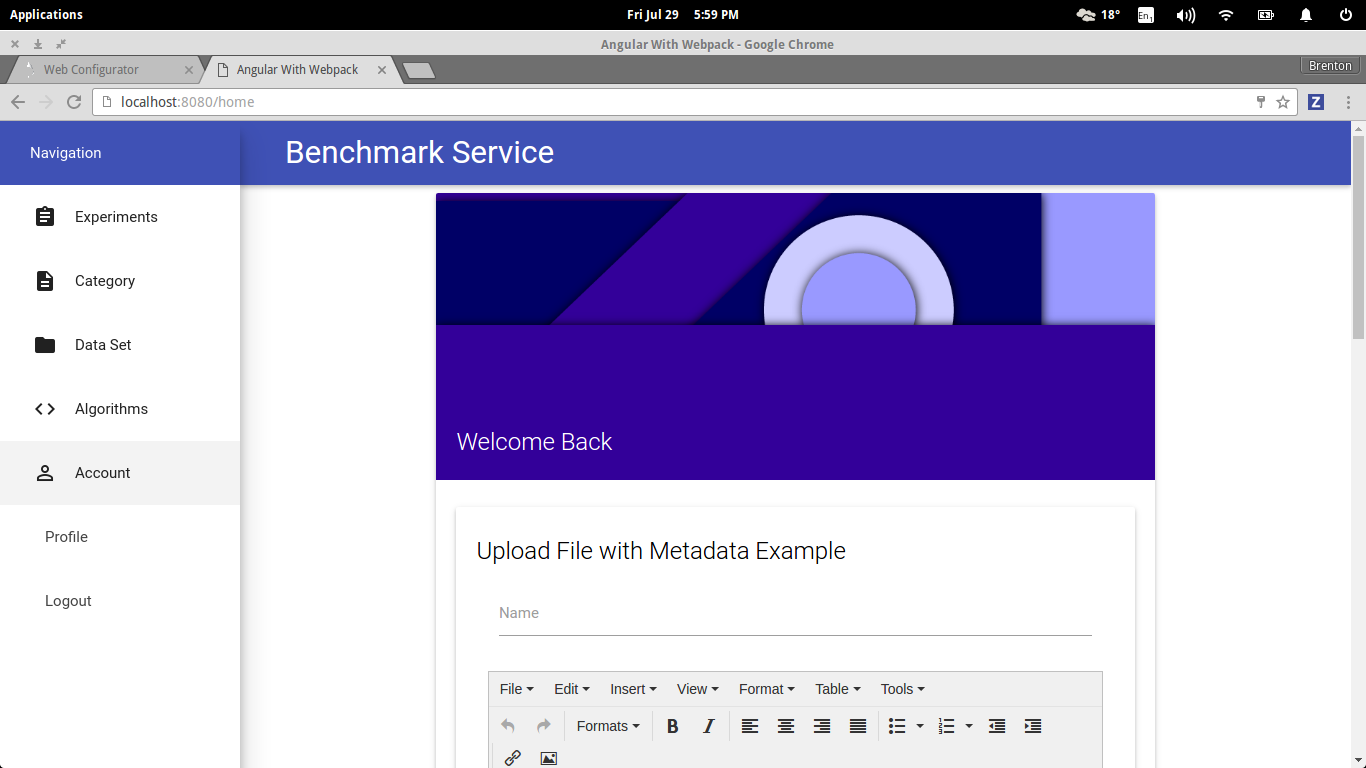
\includegraphics[scale=0.3]{../Images/User Manual/Account Page.png}
		\caption{Home Page with Account Drop down menu.}
		\label{fig:AccountPage}
	\end{center}  
\end{figure}
\begin{figure}[H]
	\begin{center}
		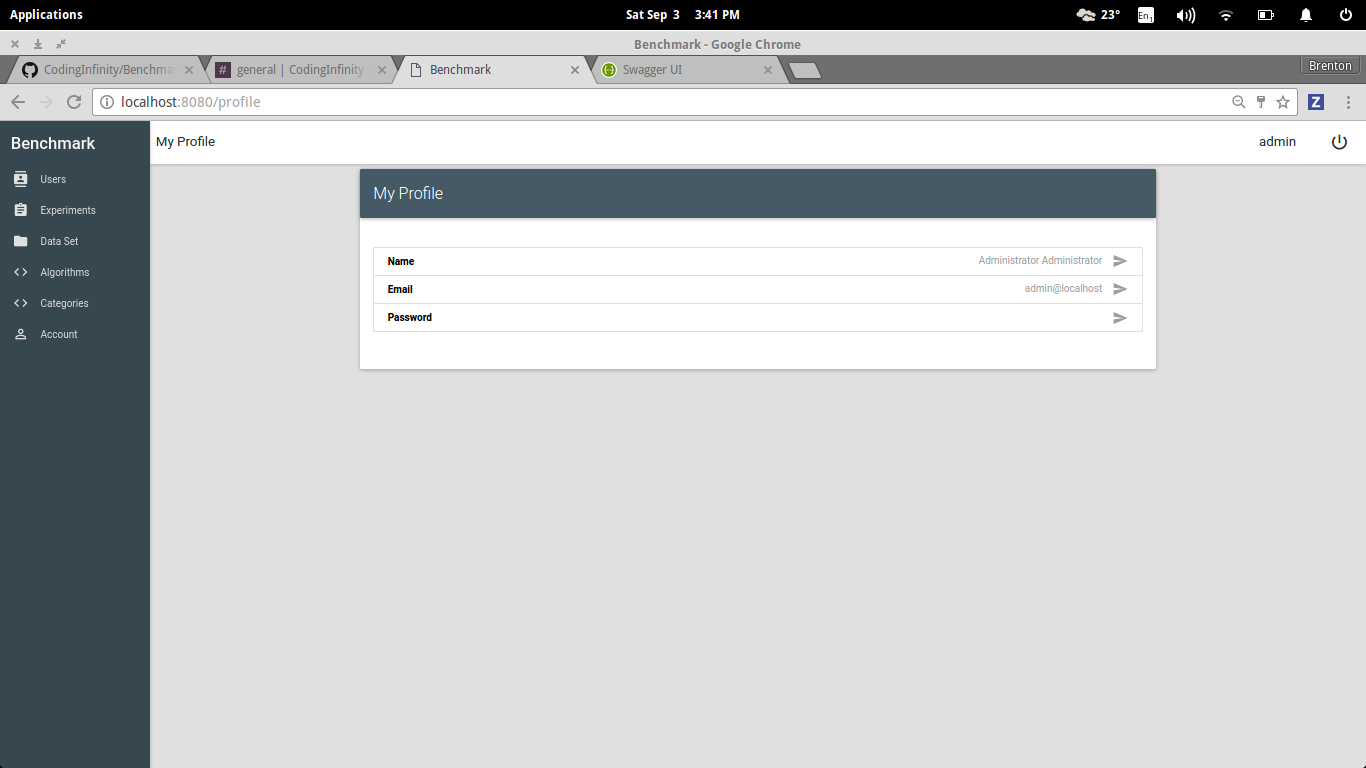
\includegraphics[scale=0.3]{../Images/User Manual/Profile Page.png}
		\caption{Profile Page}
		\label{fig:ProfilePage}
	\end{center}  
\end{figure}
\begin{figure}[H]
	\begin{center}
		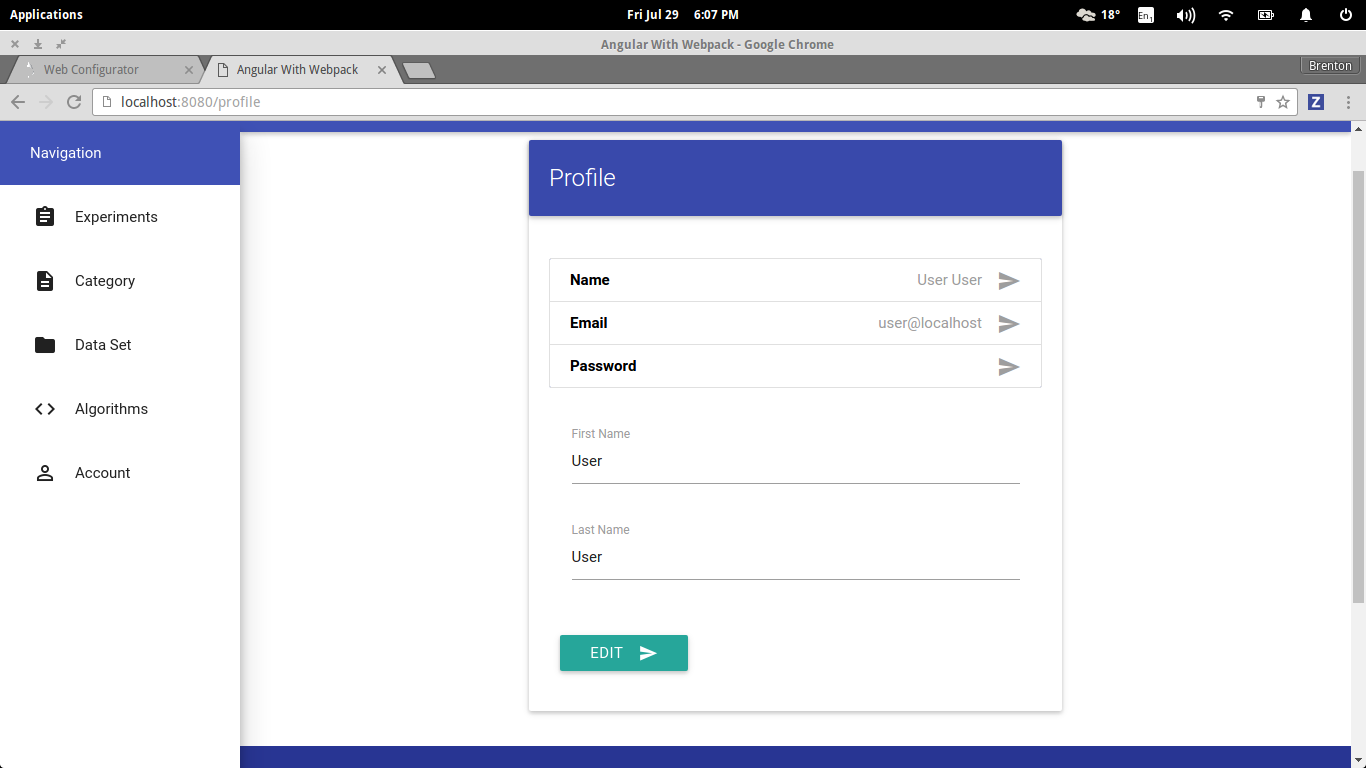
\includegraphics[scale=0.3]{../Images/User Manual/Profile Page1.png}
		\caption{Edit name}
		\label{fig:ProfilePage1}
	\end{center}  
\end{figure}
\begin{figure}[H]
	\begin{center}
		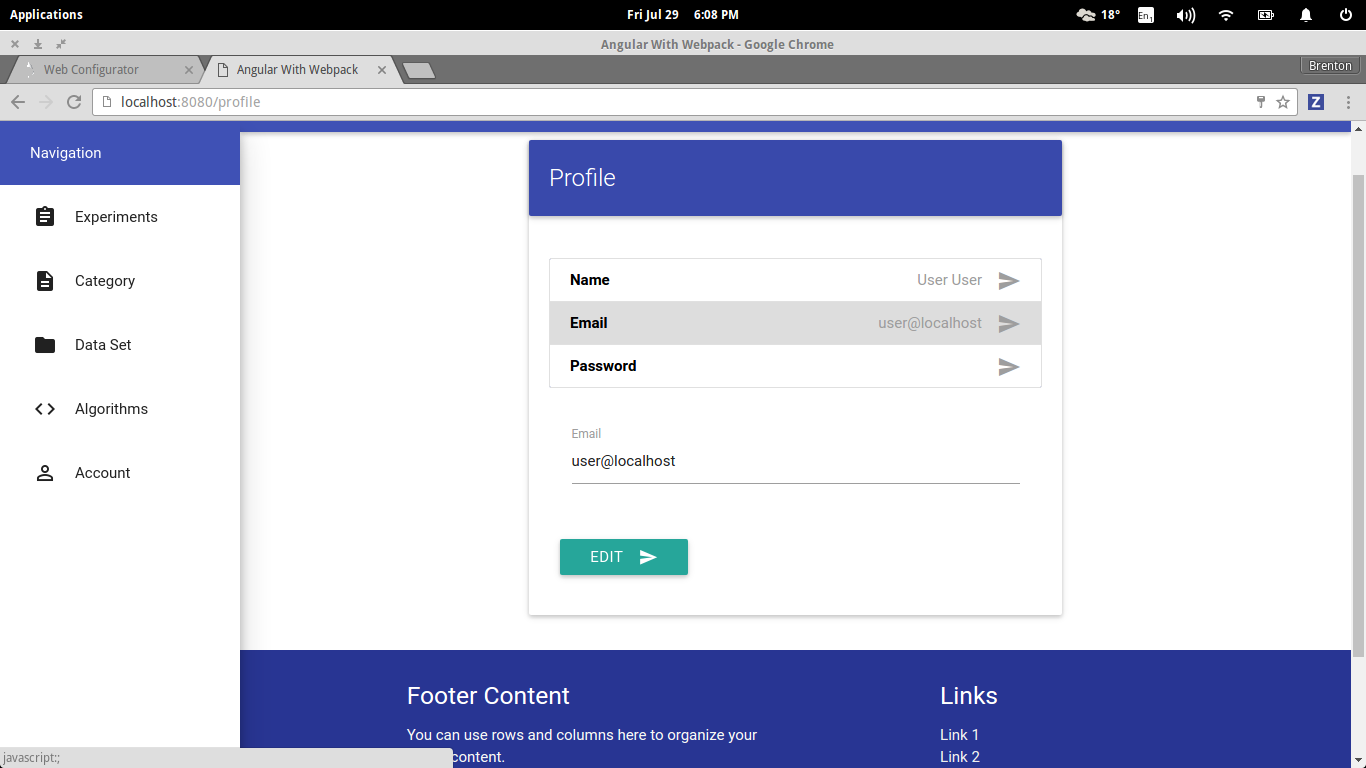
\includegraphics[scale=0.3]{../Images/User Manual/Profile Page2.png}
		\caption{Edit email}
		\label{fig:ProfilePage2}
	\end{center}  
\end{figure}
\begin{figure}[H]
	\begin{center}
		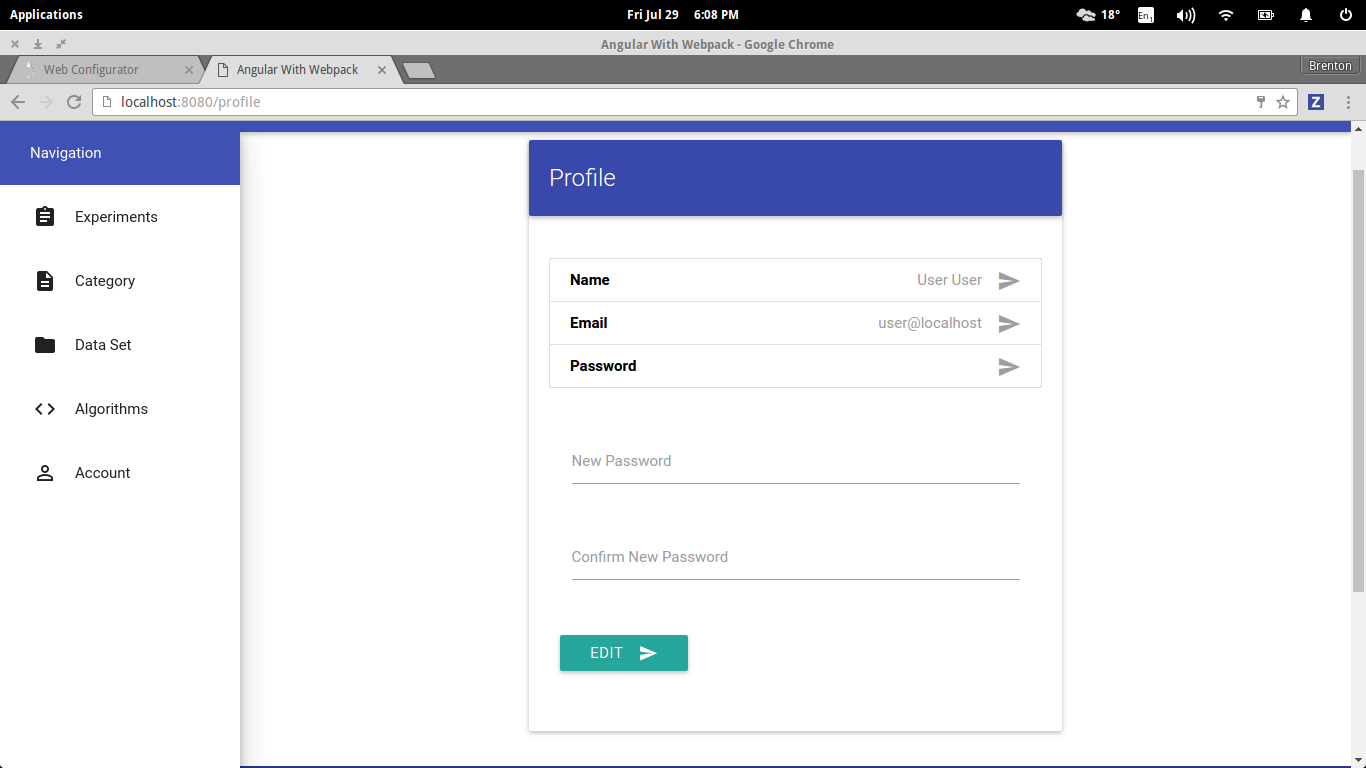
\includegraphics[scale=0.3]{../Images/User Manual/Profile Page3.png}
		\caption{Edit password}
		\label{fig:ProfilePage3}
	\end{center}  
\end{figure}

\section{Forgot password}
If one arrives at the landing page, and realizes they have lost or forgotten their password. They can select the
"Forgotten your password?" link at the bottom right which will take them to the page seen in Figure \ref{fig:forgotPage}.
\begin{figure}[H]
	\begin{center}
		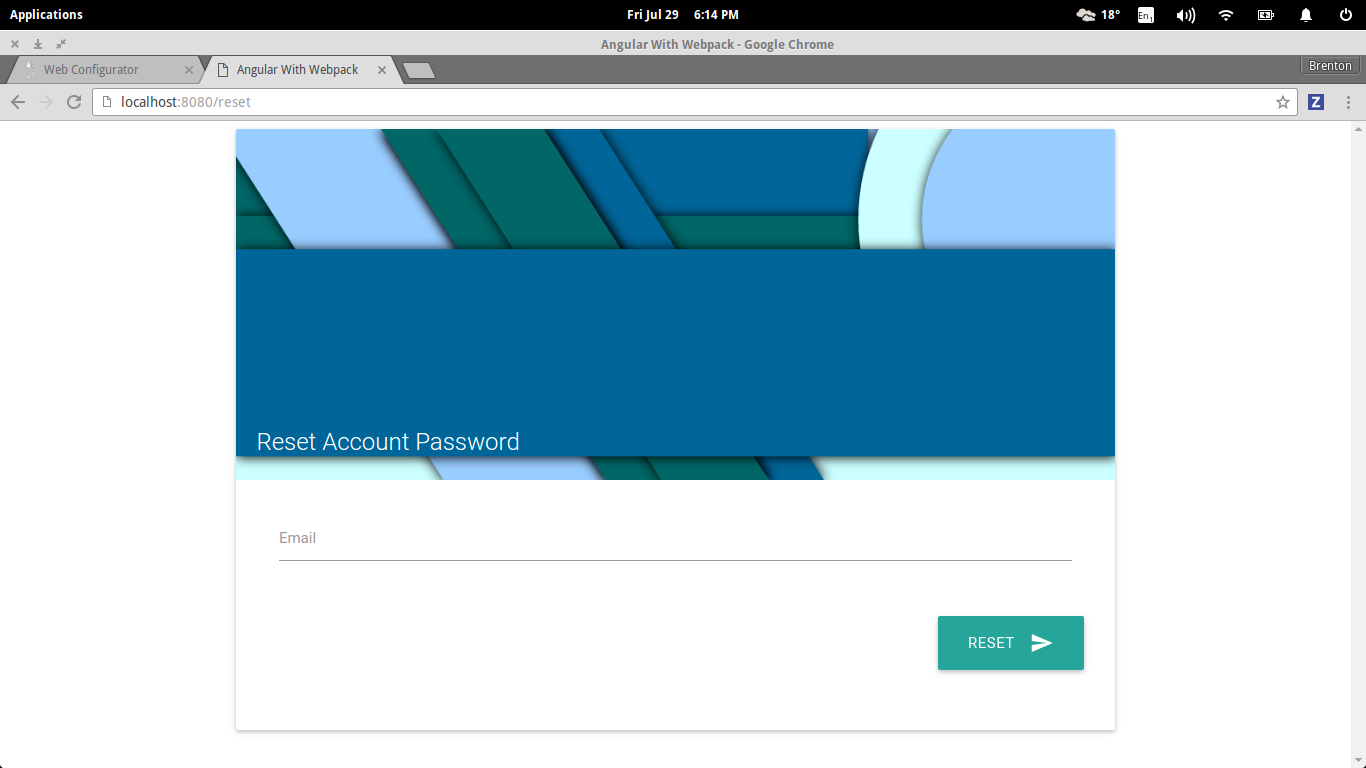
\includegraphics[scale=0.3]{../Images/User Manual/Forgot Page.png}
		\caption{Forgot password page}
		\label{fig:forgotPage}
	\end{center}  
\end{figure}
After entering their registered email address, the user will recieve an email with a link to a page to reset their password
as seen in Figure \ref{fig:resetPage}. After the user as filled in their details, the user should click "Reset".
\begin{figure}[H]
	\begin{center}
		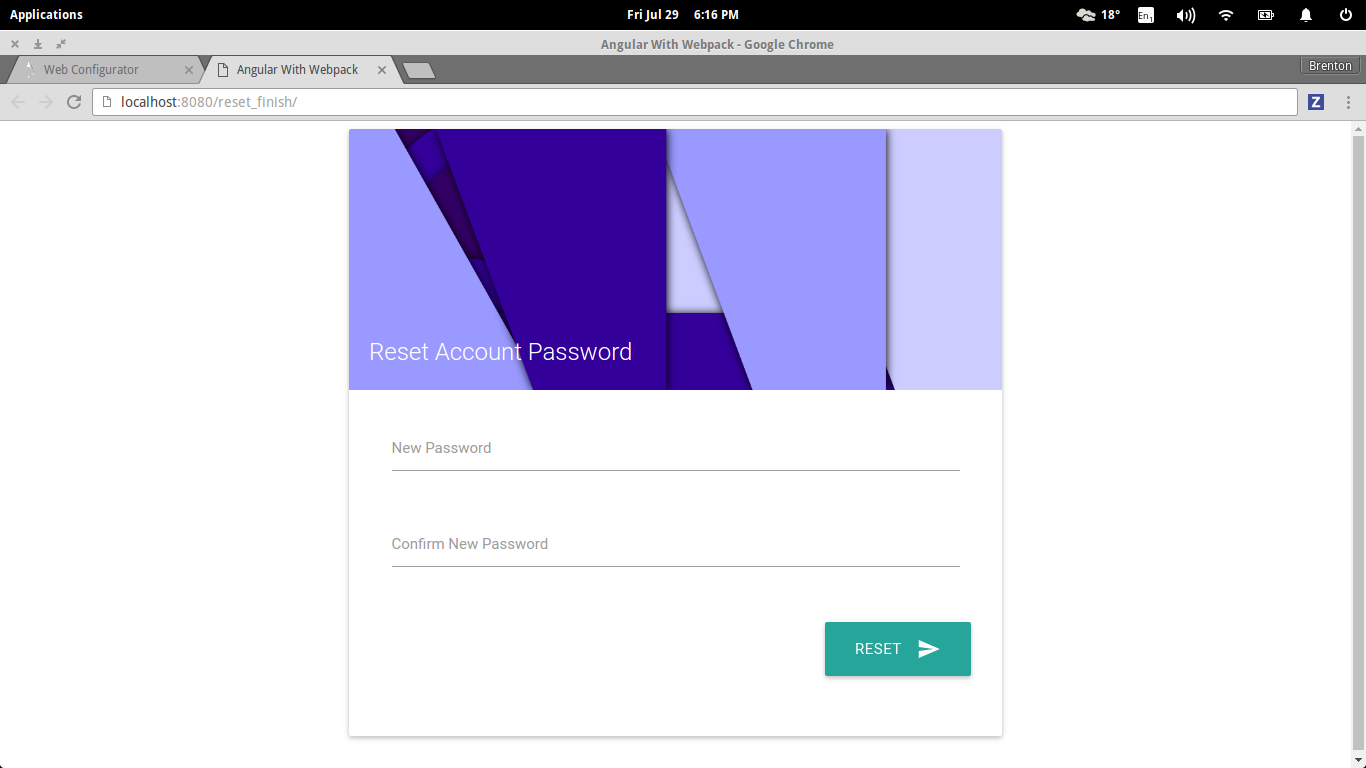
\includegraphics[scale=0.3]{../Images/User Manual/Reset Page.png}
		\caption{Reset password page}
		\label{fig:resetPage}
	\end{center}  
\end{figure}

\section{Experiment}
This section and its sub-section have not been implemented but will be in a future release.

\section{Category}
This section and its sub-section have not been implemented but will be in a future release.

\section{Dataset}
This section and its sub-section have not been implemented but will be in a future release.

\section{Algorithms}
This section and its sub-section have not been implemented but will be in a future release.
\end{document}
